% ============================================================
% CHAPITRE 4 : SPRINT 0
% Mise en place de l'environnement et Site Vitrine
% ============================================================

\section{Introduction}
Le Sprint 0, souvent appelé \textit{Sprint d'initialisation}, constitue la première itération de notre projet. Il ne produit pas de fonctionnalités métier directement visibles par l'utilisateur final, mais il pose les fondations techniques et architecturales indispensables à la réussite des sprints suivants.

Les objectifs de ce sprint sont les suivants :
\begin{itemize}
    \item Mettre en place l'environnement de développement (Frontend, Backend, Base de données).
    \item Définir l'architecture technique du projet et structurer le code source.
    \item Concevoir et développer le \textbf{site vitrine} de l'entreprise GIAS Industries (Landing Page).
    \item Configurer le système de routage, la navigation et la barre latérale (Sidebar) de l'application.
    \item Préparer la base de données MySQL et définir les modèles Sequelize avec leurs associations.
\end{itemize}

%% =======================================
%% 4.2 BACKLOG DU SPRINT 0
%% =======================================
\section{Backlog du Sprint 0}

\subsection{User Stories du Sprint 0}

\begin{center}
\begin{tabular}{|p{1cm}|p{6cm}|p{2cm}|p{5cm}|}
\hline
\textbf{ID} & \textbf{User Story} & \textbf{Priorité} & \textbf{Critères d'acceptation} \\ \hline
\textbf{US0.1} & En tant que \textbf{développeur}, je veux initialiser le projet avec les outils adéquats (React, Node.js, MySQL). & Haute & Le serveur Frontend et le serveur Backend démarrent sans erreurs. \\ \hline
\textbf{US0.2} & En tant que \textbf{visiteur}, je veux consulter un site vitrine présentant GIAS Industries. & Haute & La Landing Page est accessible et affiche les sections de l'entreprise. \\ \hline
\textbf{US0.3} & En tant que \textbf{développeur}, je veux structurer la base de données avec un ORM. & Haute & Les modèles Sequelize sont définis et les associations sont fonctionnelles. \\ \hline
\textbf{US0.4} & En tant qu'\textbf{utilisateur connecté}, je veux naviguer dans l'application via une barre latérale. & Moyenne & Le Sidebar affiche les menus selon le rôle de l'utilisateur. \\ \hline
\end{tabular}
\captionof{table}{Backlog du Sprint 0}
\end{center}

\subsection{Planification du Sprint}
La durée estimée de ce sprint est de \textbf{2 semaines}. Il couvre exclusivement la préparation de l'infrastructure technique et la création du site vitrine.

%% =======================================
%% 4.3 CONCEPTION DÉTAILLÉE
%% =======================================
\section{Conception détaillée du Sprint 0}

\subsection{Architecture globale du projet}
Le projet StageFlow adopte une architecture \textbf{3-tiers découplée} :
\begin{itemize}
    \item \textbf{Couche Présentation (Frontend)} : Application React initialisée avec \textbf{Vite.js}, utilisant \textbf{Tailwind CSS} pour le stylisme et \textbf{React Router DOM} pour la navigation.
    \item \textbf{Couche Logique (Backend)} : Serveur \textbf{Node.js} avec le framework \textbf{Express.js}, structuré selon le pattern \textit{Routes $\rightarrow$ Services $\rightarrow$ Modèles}.
    \item \textbf{Couche Données} : Base de données relationnelle \textbf{MySQL}, gérée via l'ORM \textbf{Sequelize}.
\end{itemize}

%%% --- IMAGE 1 : Architecture 3-tiers ---
%%% Remplacer IMAGE_ARCHITECTURE_3TIERS.png par le nom de ton image
\begin{center}
    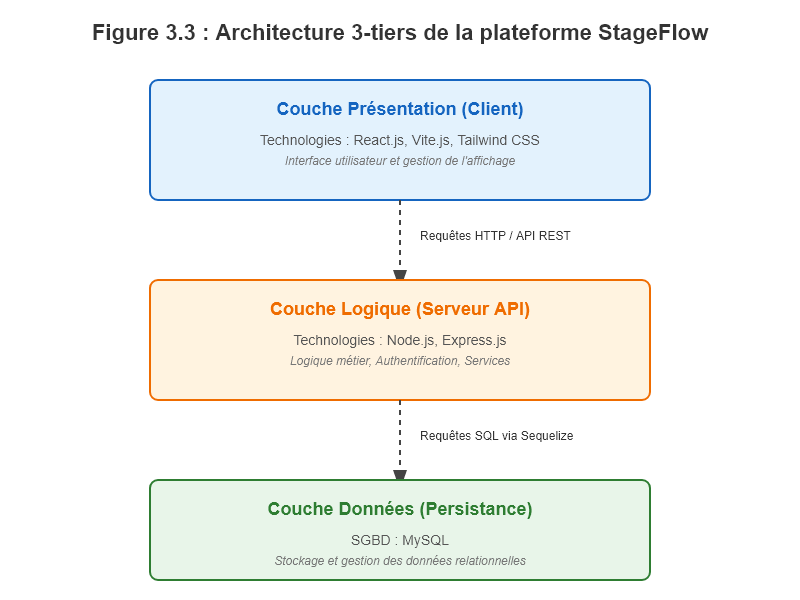
\includegraphics[width=0.8\textwidth]{IMAGE_ARCHITECTURE_3TIERS.png} \\
    \textit{\small Figure 4.1 -- Architecture 3-tiers de la plateforme StageFlow}
\end{center}

\subsection{Structure du projet}
L'arborescence du code source est organisée comme suit :

\begin{center}
\begin{tabular}{|l|p{10cm}|}
\hline
\textbf{Dossier} & \textbf{Contenu} \\ \hline
\texttt{frontend/src/pages/} & Pages principales de l'application (LandingPage, Login, Register, Dashboard, etc.) \\ \hline
\texttt{frontend/src/components/} & Composants réutilisables (Sidebar, Header, ProtectedRoute, etc.) \\ \hline
\texttt{frontend/src/components/landing/} & Composants du site vitrine (Hero, Presentation, Activites, Departements, Mission, Valeurs, Qualite, Footer) \\ \hline
\texttt{frontend/src/context/} & Gestion du contexte d'authentification (AuthContext) \\ \hline
\texttt{backend/src/routes/} & Routes API REST (auth, candidatures, departements, evaluations, etc.) \\ \hline
\texttt{backend/src/services/} & Services métier (authService, emailService, pdfService, etc.) \\ \hline
\texttt{backend/src/models/} & Modèles Sequelize (Utilisateur, Stagiaire, Candidature, Evaluation, etc.) \\ \hline
\texttt{backend/src/middleware/} & Middleware de sécurité (auth.js, rbac.js) \\ \hline
\texttt{backend/src/config/} & Configuration (database.js, company.js) \\ \hline
\end{tabular}
\captionof{table}{Structure du code source de StageFlow}
\end{center}

\subsection{Diagramme de classes global}
Le diagramme de classes suivant présente l'ensemble des entités du système et leurs relations :

%%% --- IMAGE 2 : Diagramme de classes ---
%%% Remplacer IMAGE_DIAGRAMME_CLASSES.png par le nom de ton image
\begin{center}
    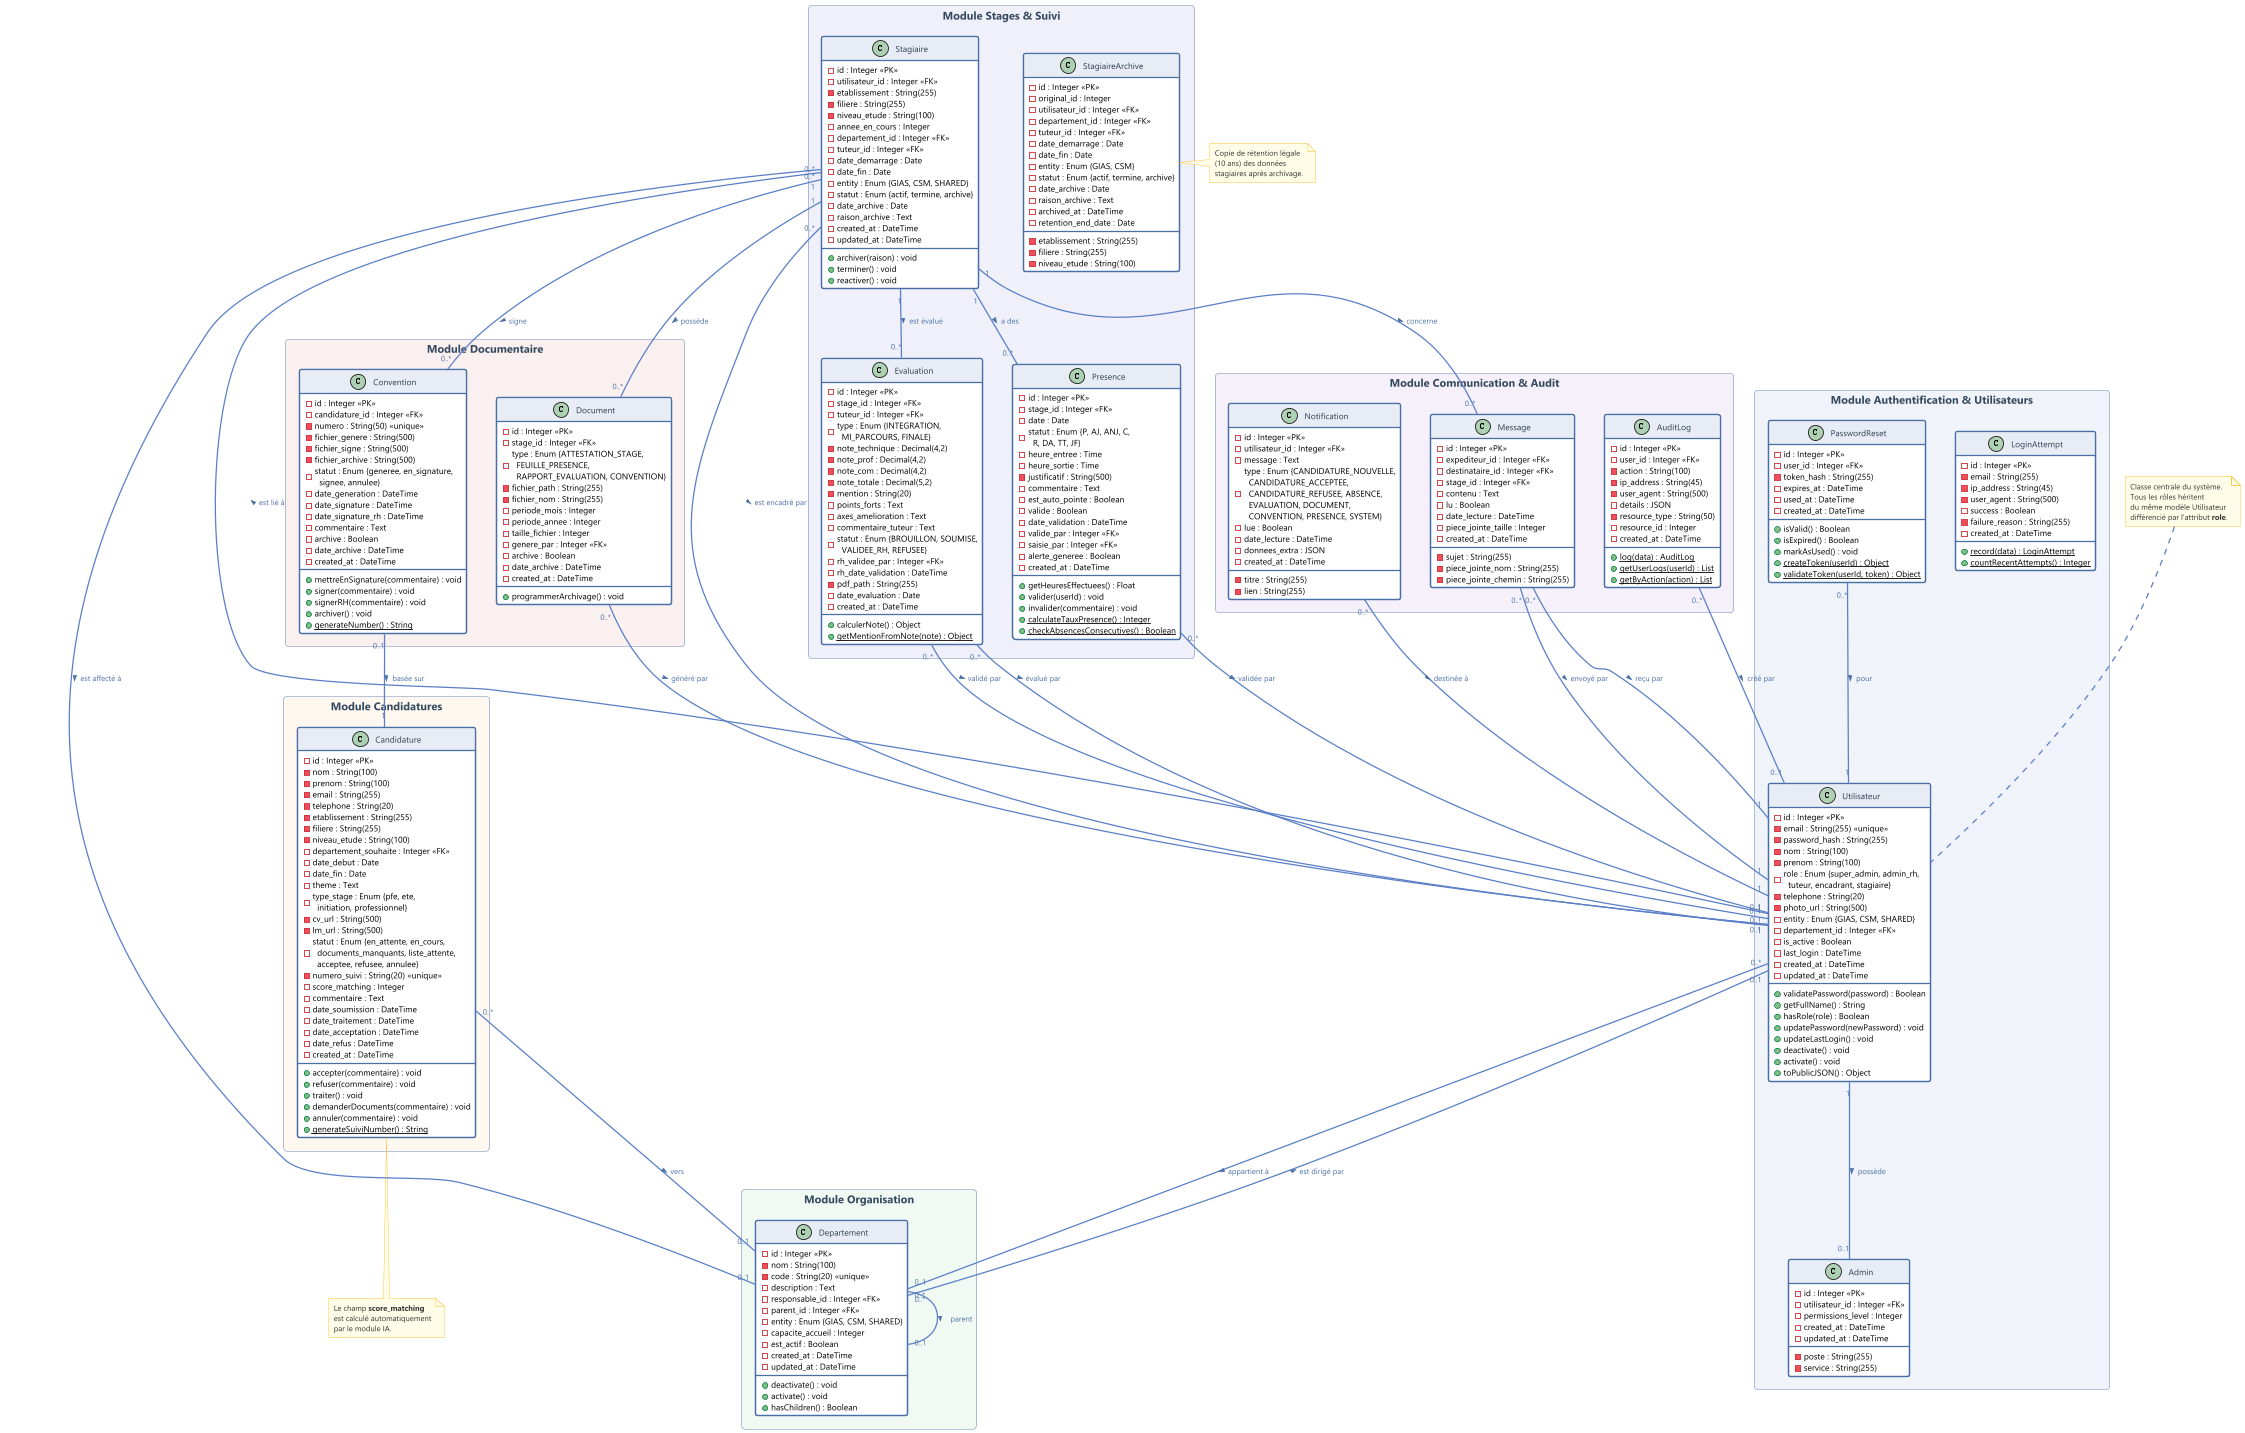
\includegraphics[width=0.9\textwidth]{IMAGE_DIAGRAMME_CLASSES.png} \\
    \textit{\small Figure 4.2 -- Diagramme de classes global de StageFlow}
\end{center}

Les principales entités du système sont :

\begin{center}
\begin{tabular}{|l|p{10cm}|}
\hline
\textbf{Entité} & \textbf{Description} \\ \hline
\texttt{Utilisateur} & Table centrale. Contient les informations de tous les acteurs (nom, prénom, email, rôle, mot de passe haché). \\ \hline
\texttt{Stagiaire} & Profil de stage associé à un utilisateur. Contient les dates de stage, le département et le tuteur assigné. \\ \hline
\texttt{Candidature} & Dossier de candidature soumis par un candidat. Contient le CV, la lettre de motivation et l'état de traitement. \\ \hline
\texttt{Departement} & Représente les départements de l'entreprise. Supporte une hiérarchie parent-enfant. \\ \hline
\texttt{Evaluation} & Fiche d'évaluation remplie par le tuteur pour évaluer les compétences du stagiaire. \\ \hline
\texttt{Presence} & Enregistrement du pointage quotidien d'un stagiaire (Présent, Absent, Retard). \\ \hline
\texttt{Convention} & Convention de stage générée automatiquement en PDF. \\ \hline
\texttt{Document} & Fichier généré par le système (attestation, convention signée). \\ \hline
\texttt{Notification} & Alerte envoyée aux utilisateurs (email ou SMS). \\ \hline
\texttt{Message} & Message interne échangé entre les acteurs du système. \\ \hline
\end{tabular}
\captionof{table}{Description des entités principales du système}
\end{center}

Les associations entre ces entités sont les suivantes :
\begin{itemize}
    \item Un \texttt{Utilisateur} peut avoir plusieurs \texttt{Stagiaires} (en tant que tuteur).
    \item Un \texttt{Stagiaire} appartient à un \texttt{Departement} et est encadré par un \texttt{Utilisateur} (tuteur).
    \item Un \texttt{Stagiaire} possède plusieurs \texttt{Evaluations}, \texttt{Presences}, \texttt{Documents} et \texttt{Conventions}.
    \item Une \texttt{Candidature} est liée à un \texttt{Departement} souhaité.
    \item Un \texttt{Departement} peut avoir un département parent (structure hiérarchique).
\end{itemize}

%% =======================================
%% 4.4 RÉALISATION ET IMPLÉMENTATION
%% =======================================
\section{Réalisation et Implémentation}

\subsection{Initialisation du Frontend}
Le frontend a été initialisé à l'aide de \textbf{Vite.js} avec le template React. Les dépendances principales installées sont :

\begin{center}
\begin{tabular}{|l|l|p{6cm}|}
\hline
\textbf{Bibliothèque} & \textbf{Version} & \textbf{Rôle} \\ \hline
\texttt{react} & 18.2.0 & Bibliothèque d'interface utilisateur \\ \hline
\texttt{react-router-dom} & 6.21.1 & Gestion du routage côté client \\ \hline
\texttt{axios} & 1.6.5 & Client HTTP pour les appels API \\ \hline
\texttt{tailwindcss} & 4.2.2 & Framework CSS utilitaire \\ \hline
\texttt{zustand} & 4.4.7 & Gestion d'état légère \\ \hline
\texttt{react-hook-form} & 7.49.2 & Gestion des formulaires \\ \hline
\texttt{zod} & 3.22.4 & Validation de schéma de données \\ \hline
\texttt{d3} & 7.9.0 & Visualisation de données et graphiques \\ \hline
\texttt{lucide-react} & 0.303.0 & Bibliothèque d'icônes modernes \\ \hline
\texttt{jspdf} & 4.2.0 & Génération de PDF côté client \\ \hline
\end{tabular}
\captionof{table}{Dépendances principales du Frontend}
\end{center}

\subsection{Initialisation du Backend}
Le backend a été configuré avec \textbf{Node.js} (version 18+) et \textbf{Express.js}. Les dépendances principales sont :

\begin{center}
\begin{tabular}{|l|l|p{6cm}|}
\hline
\textbf{Bibliothèque} & \textbf{Version} & \textbf{Rôle} \\ \hline
\texttt{express} & 4.18.2 & Framework web HTTP \\ \hline
\texttt{sequelize} & 6.35.2 & ORM pour MySQL \\ \hline
\texttt{mysql2} & 3.6.5 & Pilote de connexion MySQL \\ \hline
\texttt{jsonwebtoken} & 9.0.2 & Génération et vérification des tokens JWT \\ \hline
\texttt{bcrypt} & 5.1.1 & Hachage sécurisé des mots de passe \\ \hline
\texttt{nodemailer} & 8.0.4 & Envoi d'emails (OTP, notifications) \\ \hline
\texttt{helmet} & 7.1.0 & Sécurisation des en-têtes HTTP \\ \hline
\texttt{express-rate-limit} & 7.1.5 & Protection contre les attaques par force brute \\ \hline
\texttt{multer} & 2.1.1 & Gestion de l'upload de fichiers \\ \hline
\texttt{pdfkit} & 0.17.2 & Génération de documents PDF côté serveur \\ \hline
\texttt{cors} & 2.8.5 & Gestion des requêtes Cross-Origin \\ \hline
\end{tabular}
\captionof{table}{Dépendances principales du Backend}
\end{center}

\subsection{Configuration de la base de données}
La base de données \textbf{MySQL} a été configurée via Sequelize avec les paramètres suivants :
\begin{itemize}
    \item \textbf{Nom de la base} : \texttt{gestion\_stagiaires}
    \item \textbf{Pool de connexions} : Maximum 10 connexions simultanées
    \item \textbf{Charset} : \texttt{utf8mb4\_unicode\_ci} pour le support complet des caractères Unicode
    \item \textbf{Timestamps automatiques} : Chaque table possède les champs \texttt{created\_at} et \texttt{updated\_at}
\end{itemize}

\subsection{Développement du site vitrine (Landing Page)}
Le site vitrine constitue le premier point de contact entre le visiteur et la plateforme StageFlow. Il présente l'entreprise GIAS Industries et invite les candidats à postuler.

La Landing Page est composée de \textbf{9 composants React} organisés verticalement :

\begin{center}
\begin{tabular}{|p{1cm}|l|p{8cm}|}
\hline
\textbf{N\textsuperscript{o}} & \textbf{Composant} & \textbf{Description} \\ \hline
1 & \texttt{Header} & Barre de navigation fixe avec le logo GIAS, les liens de navigation et les boutons ``Se connecter'' et ``Rejoindre''. Elle devient semi-transparente avec un effet de flou (glassmorphism) au défilement. \\ \hline
2 & \texttt{Hero} & Section d'accroche principale avec le titre ``L'Art des Ingrédients'', un bouton d'inscription, un bouton de connexion et un champ de suivi de candidature. \\ \hline
3 & \texttt{Presentation} & Présentation de l'entreprise avec une image et un badge de certification ISO. \\ \hline
4 & \texttt{Activites} & Trois cartes interactives présentant les activités : Margarines, Chocolat et Mixes. \\ \hline
5 & \texttt{Departements} & Présentation des départements de l'entreprise. \\ \hline
6 & \texttt{Mission} & Énoncé de la mission de GIAS Industries. \\ \hline
7 & \texttt{Valeurs} & Présentation des valeurs fondamentales de l'entreprise. \\ \hline
8 & \texttt{Qualite} & Section dédiée aux standards de qualité et aux certifications. \\ \hline
9 & \texttt{Footer} & Pied de page avec les coordonnées, les liens rapides et les réseaux sociaux. \\ \hline
\end{tabular}
\captionof{table}{Composants du site vitrine}
\end{center}

Des animations au défilement (\textit{scroll reveal}) ont été implémentées via l'API \texttt{IntersectionObserver} pour donner une impression de dynamisme à la page.

\subsection{Mise en place du système de navigation (Sidebar)}
La barre latérale de l'application affiche les menus de navigation en fonction du rôle de l'utilisateur connecté. Les rôles supportés sont :

\begin{center}
\begin{tabular}{|l|l|p{6cm}|}
\hline
\textbf{Rôle} & \textbf{Libellé affiché} & \textbf{Accès aux modules} \\ \hline
\texttt{admin\_rh} & Admin RH & Tableau de bord, Stagiaires, Candidatures, Départements, Présences, Évaluations, Documents, Notifications \\ \hline
\texttt{tuteur} & Tuteur & Tableau de bord, Stagiaires, Présences, Évaluations, Notifications \\ \hline
\texttt{stagiaire} & Stagiaire & Mon Espace, Ma Présence, Mes Évaluations, Notifications \\ \hline
\end{tabular}
\captionof{table}{Accès par rôle dans la barre latérale}
\end{center}

\subsection{Configuration des routes API}
Le point d'entrée du backend (\texttt{index.js}) configure les \textbf{12 routes API REST} suivantes :

\begin{center}
\begin{tabular}{|l|l|}
\hline
\textbf{Route} & \textbf{Module} \\ \hline
\texttt{/api/auth} & Authentification (Inscription, Connexion, OTP) \\ \hline
\texttt{/api/users} & Gestion des utilisateurs \\ \hline
\texttt{/api/departements} & Gestion des départements \\ \hline
\texttt{/api/tuteurs} & Gestion des tuteurs \\ \hline
\texttt{/api/candidatures} & Gestion des candidatures \\ \hline
\texttt{/api/conventions} & Gestion des conventions de stage \\ \hline
\texttt{/api/presences} & Gestion des présences \\ \hline
\texttt{/api/evaluations} & Gestion des évaluations \\ \hline
\texttt{/api/documents} & Gestion des documents \\ \hline
\texttt{/api/dashboard} & Statistiques et tableau de bord \\ \hline
\texttt{/api/notifications} & Notifications et messagerie \\ \hline
\texttt{/api/stagiaires} & Gestion et recherche de stagiaires \\ \hline
\end{tabular}
\captionof{table}{Routes API REST de StageFlow}
\end{center}

Les middlewares de sécurité configurés globalement sont :
\begin{itemize}
    \item \textbf{CORS} : Autorise les requêtes depuis les ports de développement (5173, 5174, 5175).
    \item \textbf{Helmet} : Sécurise les en-têtes HTTP de chaque réponse.
    \item \textbf{Rate Limiting} : Limite à 100 requêtes par minute par IP.
    \item \textbf{Morgan} : Journalisation de toutes les requêtes HTTP entrantes.
\end{itemize}

%% =======================================
%% 4.5 PRÉSENTATION DES INTERFACES
%% =======================================
\section{Présentation des interfaces}
Cette section illustre les résultats visuels obtenus à l'issue du Sprint 0.

\subsection{Page d'accueil -- Section Hero}
La section Hero est la première chose que voit le visiteur. Elle affiche le titre ``L'Art des Ingrédients'' avec des boutons d'inscription et de connexion.

%%% --- IMAGE 3 : Capture Hero ---
%%% Remplacer IMAGE_CAPTURE_HERO.png par le nom de ta capture d'écran
\begin{center}
    \includegraphics[width=0.85\textwidth]{IMAGE_CAPTURE_HERO.png} \\
    \textit{\small Figure 4.3 -- Section Hero de la Landing Page}
\end{center}

\subsection{Page d'accueil -- Section Présentation}
Cette section présente l'entreprise GIAS Industries avec une image et un badge de certification ISO.

%%% --- IMAGE 4 : Capture Présentation ---
%%% Remplacer IMAGE_CAPTURE_PRESENTATION.png par le nom de ta capture d'écran
\begin{center}
    \includegraphics[width=0.85\textwidth]{IMAGE_CAPTURE_PRESENTATION.png} \\
    \textit{\small Figure 4.4 -- Section Présentation de l'entreprise}
\end{center}

\subsection{Page d'accueil -- Section Activités}
Trois cartes interactives présentent les activités principales : Margarines, Chocolat et Mixes.

%%% --- IMAGE 5 : Capture Activités ---
%%% Remplacer IMAGE_CAPTURE_ACTIVITES.png par le nom de ta capture d'écran
\begin{center}
    \includegraphics[width=0.85\textwidth]{IMAGE_CAPTURE_ACTIVITES.png} \\
    \textit{\small Figure 4.5 -- Section Activités de GIAS Industries}
\end{center}

\subsection{Page d'accueil -- Footer}
Le pied de page contient les coordonnées de l'entreprise, les liens de candidature et les réseaux sociaux.

%%% --- IMAGE 6 : Capture Footer ---
%%% Remplacer IMAGE_CAPTURE_FOOTER.png par le nom de ta capture d'écran
\begin{center}
    \includegraphics[width=0.85\textwidth]{IMAGE_CAPTURE_FOOTER.png} \\
    \textit{\small Figure 4.6 -- Pied de page du site vitrine}
\end{center}

\subsection{Barre latérale de navigation (Sidebar)}
La barre latérale affiche les modules accessibles selon le rôle de l'utilisateur connecté.

%%% --- IMAGE 7 : Capture Sidebar ---
%%% Remplacer IMAGE_CAPTURE_SIDEBAR.png par le nom de ta capture d'écran
\begin{center}
    \includegraphics[width=0.3\textwidth]{IMAGE_CAPTURE_SIDEBAR.png} \\
    \textit{\small Figure 4.7 -- Barre latérale de l'application (vue Admin RH)}
\end{center}

%% =======================================
%% 4.6 TESTS ET VALIDATION
%% =======================================
\section{Tests et Validation du Sprint 0}
Les tests suivants ont été réalisés pour valider le bon fonctionnement de l'infrastructure mise en place :

\begin{center}
\begin{tabular}{|p{1cm}|p{5cm}|p{4cm}|p{3cm}|}
\hline
\textbf{ID} & \textbf{Scénario de test} & \textbf{Résultat attendu} & \textbf{Statut} \\ \hline
T0.1 & Démarrage du serveur Backend & Le serveur démarre sur le port 3000 sans erreurs. & \textcolor{green}{Validé} \\ \hline
T0.2 & Démarrage du serveur Frontend & L'application React est accessible sur le port 5173. & \textcolor{green}{Validé} \\ \hline
T0.3 & Connexion à la base de données MySQL & Le message ``DB connectée'' s'affiche dans la console. & \textcolor{green}{Validé} \\ \hline
T0.4 & Chargement de la Landing Page & La page d'accueil s'affiche correctement avec toutes les sections. & \textcolor{green}{Validé} \\ \hline
T0.5 & Navigation responsive & Le site est correctement affiché sur mobile et tablette. & \textcolor{green}{Validé} \\ \hline
T0.6 & Vérification du endpoint santé & L'appel \texttt{GET /health} retourne \texttt{\{status: "ok"\}}. & \textcolor{green}{Validé} \\ \hline
\end{tabular}
\captionof{table}{Résultats des tests du Sprint 0}
\end{center}

%% =======================================
%% 4.7 CONCLUSION
%% =======================================
\section{Conclusion du Sprint 0}
Le Sprint 0 a été achevé avec succès. L'environnement de développement est entièrement opérationnel, le site vitrine de GIAS Industries est en ligne, et l'architecture technique est prête pour accueillir les fonctionnalités métiers des prochains sprints. La base de données MySQL est configurée avec \textbf{10 modèles Sequelize} et leurs associations sont fonctionnelles.

Le prochain sprint (Sprint 1) sera consacré à la mise en place du système d'authentification sécurisé et de la gestion des utilisateurs.
